\section{Finding 13 - Possible SYN Flood Attack}
%center under chapter title a one row table with 6 coloumns and no borders
\vspace*{-0,3cm}
\begin{center}
    \begin{tabular}{c c c c}
        \textbf{Classification:} & Denial of Service & \textbf{Severity:} & \textbf{\textcolor{orange}{Medium}}  
        \end{tabular}
\end{center}
The \ac{DUT} is vulnerable to a SYN flood attack.


\subsection*{Finding Impact}
This lead to a denial of service attack on the \ac{DUT}.

\subsection*{Finding Details}
Following command has been executed on the \ac{DUT}:
\begin{lstlisting}
sudo hping3 -c 15000 -d 120 -S -w 64 -p 80 -flood 
--rand-source 172.16.0.29
\end{lstlisting}
The attack can be analized within Wireshark:
%image
\begin{figure}[H]
    \centering
    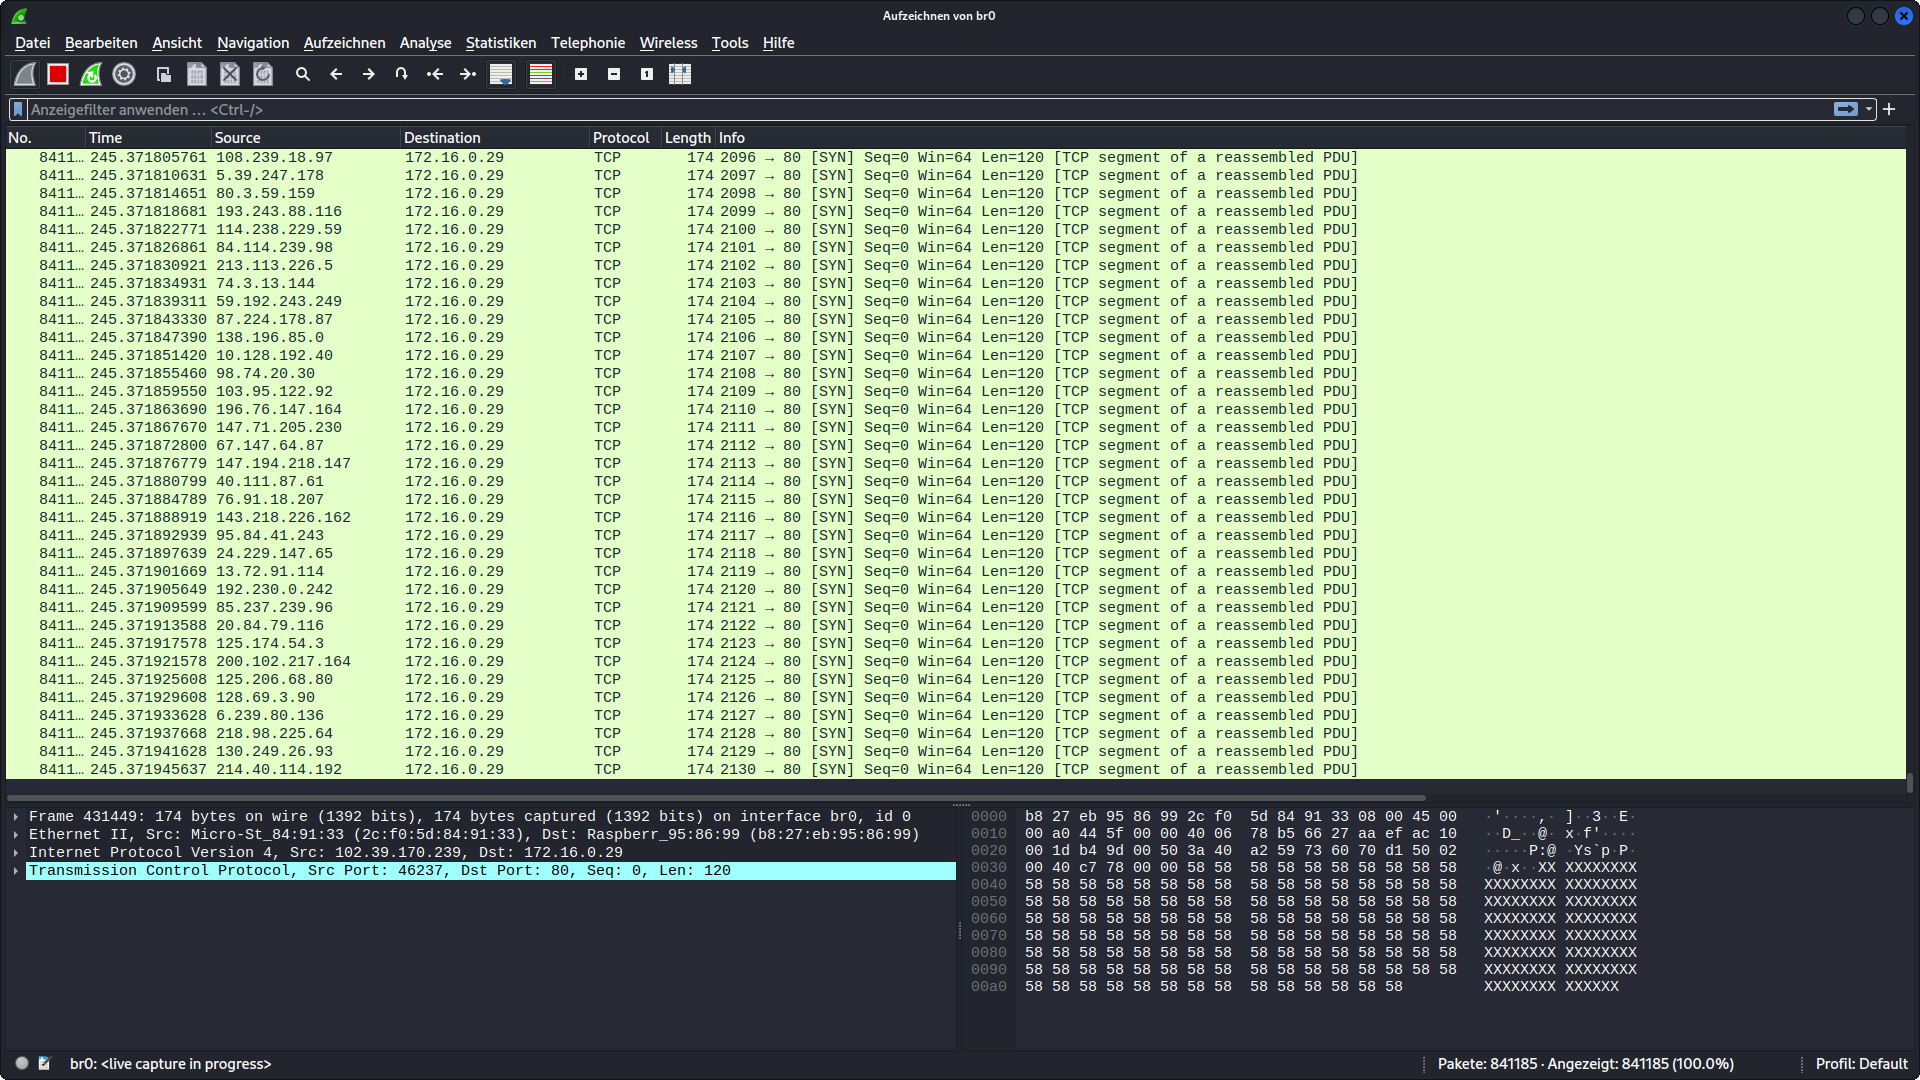
\includegraphics[width=1\textwidth]{img/syn-flooding.png}
    \caption{Wireshark}
    \label{fig:fin13}
\end{figure}

\subsection*{Evaluation of Results}
\begin{center}
    \begin{tabular}{cccc}
    \textbf{Effort to Fix:} & &\ \textbf{\textcolor{red}{High}}\
    \end{tabular}
\end{center}
To prevent SYN flood attacks a \ac{IPS} could be implemented. Also external services against \ac{DDoS} attacks in general could be used.
